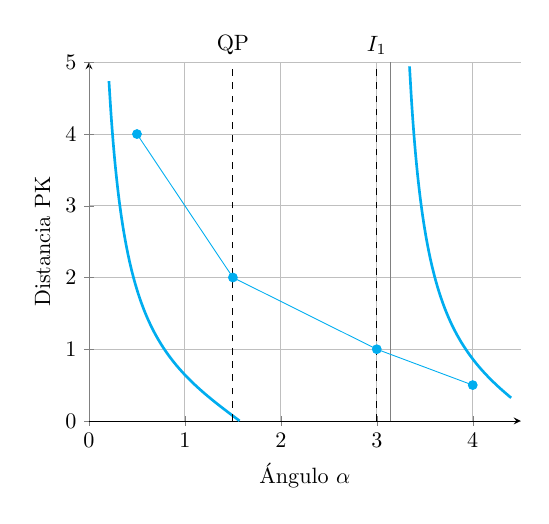
\begin{tikzpicture}[scale=0.8]
\begin{axis}[
    xlabel={Ángulo $\alpha$},
    ylabel={Distancia PK},
    xmin=0, xmax=4.5,
    ymin=0, ymax=5,
    grid=major,
    axis lines=left,
    samples=200,
    domain=0.1:4.4,
    restrict y to domain=0:5,
    clip=false
]

% Función cotangente principal (azul/cyan)
\addplot[cyan, very thick, smooth, unbounded coords=jump] {
    (x > 0.05 && x < 3.09) ? (1/tan(deg(x))) : 
    (x > 3.19 && x < 6.23) ? (1/tan(deg(x))) : nan
};

% Líneas punteadas verticales
\draw[dashed, black] (axis cs:1.5,0) -- (axis cs:1.5,5) node[above] {QP};
\draw[dashed, black] (axis cs:3.0,0) -- (axis cs:3.0,5) node[above] {$I_1$};

% Asíntotas verticales
\draw[gray, very thin] (axis cs:0,0) -- (axis cs:0,5);
\draw[gray, very thin] (axis cs:3.14159,0) -- (axis cs:3.14159,5);

% Puntos importantes
\addplot[cyan, mark=*, mark size=2pt] coordinates {(0.5,4) (1.5,2) (3.0,1) (4.0,0.5)};

\end{axis}
\end{tikzpicture}
